% Options for packages loaded elsewhere
\PassOptionsToPackage{unicode}{hyperref}
\PassOptionsToPackage{hyphens}{url}
%
\documentclass[
]{article}
\usepackage{amsmath,amssymb}
\usepackage{iftex}
\ifPDFTeX
  \usepackage[T1]{fontenc}
  \usepackage[utf8]{inputenc}
  \usepackage{textcomp} % provide euro and other symbols
\else % if luatex or xetex
  \usepackage{unicode-math} % this also loads fontspec
  \defaultfontfeatures{Scale=MatchLowercase}
  \defaultfontfeatures[\rmfamily]{Ligatures=TeX,Scale=1}
\fi
\usepackage{lmodern}
\ifPDFTeX\else
  % xetex/luatex font selection
\fi
% Use upquote if available, for straight quotes in verbatim environments
\IfFileExists{upquote.sty}{\usepackage{upquote}}{}
\IfFileExists{microtype.sty}{% use microtype if available
  \usepackage[]{microtype}
  \UseMicrotypeSet[protrusion]{basicmath} % disable protrusion for tt fonts
}{}
\makeatletter
\@ifundefined{KOMAClassName}{% if non-KOMA class
  \IfFileExists{parskip.sty}{%
    \usepackage{parskip}
  }{% else
    \setlength{\parindent}{0pt}
    \setlength{\parskip}{6pt plus 2pt minus 1pt}}
}{% if KOMA class
  \KOMAoptions{parskip=half}}
\makeatother
\usepackage{xcolor}
\usepackage[margin=1in]{geometry}
\usepackage{color}
\usepackage{fancyvrb}
\newcommand{\VerbBar}{|}
\newcommand{\VERB}{\Verb[commandchars=\\\{\}]}
\DefineVerbatimEnvironment{Highlighting}{Verbatim}{commandchars=\\\{\}}
% Add ',fontsize=\small' for more characters per line
\usepackage{framed}
\definecolor{shadecolor}{RGB}{248,248,248}
\newenvironment{Shaded}{\begin{snugshade}}{\end{snugshade}}
\newcommand{\AlertTok}[1]{\textcolor[rgb]{0.94,0.16,0.16}{#1}}
\newcommand{\AnnotationTok}[1]{\textcolor[rgb]{0.56,0.35,0.01}{\textbf{\textit{#1}}}}
\newcommand{\AttributeTok}[1]{\textcolor[rgb]{0.13,0.29,0.53}{#1}}
\newcommand{\BaseNTok}[1]{\textcolor[rgb]{0.00,0.00,0.81}{#1}}
\newcommand{\BuiltInTok}[1]{#1}
\newcommand{\CharTok}[1]{\textcolor[rgb]{0.31,0.60,0.02}{#1}}
\newcommand{\CommentTok}[1]{\textcolor[rgb]{0.56,0.35,0.01}{\textit{#1}}}
\newcommand{\CommentVarTok}[1]{\textcolor[rgb]{0.56,0.35,0.01}{\textbf{\textit{#1}}}}
\newcommand{\ConstantTok}[1]{\textcolor[rgb]{0.56,0.35,0.01}{#1}}
\newcommand{\ControlFlowTok}[1]{\textcolor[rgb]{0.13,0.29,0.53}{\textbf{#1}}}
\newcommand{\DataTypeTok}[1]{\textcolor[rgb]{0.13,0.29,0.53}{#1}}
\newcommand{\DecValTok}[1]{\textcolor[rgb]{0.00,0.00,0.81}{#1}}
\newcommand{\DocumentationTok}[1]{\textcolor[rgb]{0.56,0.35,0.01}{\textbf{\textit{#1}}}}
\newcommand{\ErrorTok}[1]{\textcolor[rgb]{0.64,0.00,0.00}{\textbf{#1}}}
\newcommand{\ExtensionTok}[1]{#1}
\newcommand{\FloatTok}[1]{\textcolor[rgb]{0.00,0.00,0.81}{#1}}
\newcommand{\FunctionTok}[1]{\textcolor[rgb]{0.13,0.29,0.53}{\textbf{#1}}}
\newcommand{\ImportTok}[1]{#1}
\newcommand{\InformationTok}[1]{\textcolor[rgb]{0.56,0.35,0.01}{\textbf{\textit{#1}}}}
\newcommand{\KeywordTok}[1]{\textcolor[rgb]{0.13,0.29,0.53}{\textbf{#1}}}
\newcommand{\NormalTok}[1]{#1}
\newcommand{\OperatorTok}[1]{\textcolor[rgb]{0.81,0.36,0.00}{\textbf{#1}}}
\newcommand{\OtherTok}[1]{\textcolor[rgb]{0.56,0.35,0.01}{#1}}
\newcommand{\PreprocessorTok}[1]{\textcolor[rgb]{0.56,0.35,0.01}{\textit{#1}}}
\newcommand{\RegionMarkerTok}[1]{#1}
\newcommand{\SpecialCharTok}[1]{\textcolor[rgb]{0.81,0.36,0.00}{\textbf{#1}}}
\newcommand{\SpecialStringTok}[1]{\textcolor[rgb]{0.31,0.60,0.02}{#1}}
\newcommand{\StringTok}[1]{\textcolor[rgb]{0.31,0.60,0.02}{#1}}
\newcommand{\VariableTok}[1]{\textcolor[rgb]{0.00,0.00,0.00}{#1}}
\newcommand{\VerbatimStringTok}[1]{\textcolor[rgb]{0.31,0.60,0.02}{#1}}
\newcommand{\WarningTok}[1]{\textcolor[rgb]{0.56,0.35,0.01}{\textbf{\textit{#1}}}}
\usepackage{graphicx}
\makeatletter
\def\maxwidth{\ifdim\Gin@nat@width>\linewidth\linewidth\else\Gin@nat@width\fi}
\def\maxheight{\ifdim\Gin@nat@height>\textheight\textheight\else\Gin@nat@height\fi}
\makeatother
% Scale images if necessary, so that they will not overflow the page
% margins by default, and it is still possible to overwrite the defaults
% using explicit options in \includegraphics[width, height, ...]{}
\setkeys{Gin}{width=\maxwidth,height=\maxheight,keepaspectratio}
% Set default figure placement to htbp
\makeatletter
\def\fps@figure{htbp}
\makeatother
\setlength{\emergencystretch}{3em} % prevent overfull lines
\providecommand{\tightlist}{%
  \setlength{\itemsep}{0pt}\setlength{\parskip}{0pt}}
\setcounter{secnumdepth}{-\maxdimen} % remove section numbering
\ifLuaTeX
  \usepackage{selnolig}  % disable illegal ligatures
\fi
\usepackage{bookmark}
\IfFileExists{xurl.sty}{\usepackage{xurl}}{} % add URL line breaks if available
\urlstyle{same}
\hypersetup{
  pdftitle={Project for Assignment 3},
  hidelinks,
  pdfcreator={LaTeX via pandoc}}

\title{Project for Assignment 3}
\author{}
\date{\vspace{-2.5em}2024-11-13}

\begin{document}
\maketitle

\subsection{Question 1}\label{question-1}

Creating the Scatter Plot: The black dots are considered Diabetes level
0 while red dots are considered Diabetes level 1.

\begin{enumerate}
\def\labelenumi{\arabic{enumi}.}
\tightlist
\item
  Do you think that Diabetes is easy to classify by a standard logistic
  regression model that uses these two variables as features?
\end{enumerate}

We do not believe that Diabetes is easy to classify by a standard
logistic regression model that uses only two variables (Age and Glucose
Concentration) as features. If we look at the plot
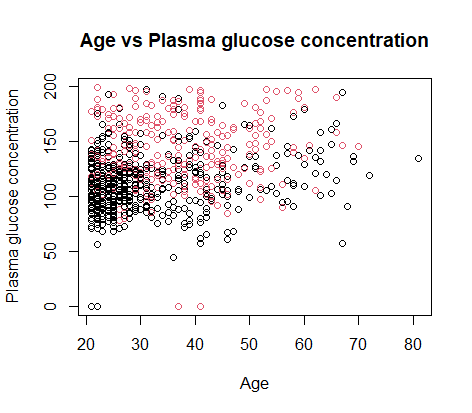
\includegraphics{"C:/Users/Ana/Documents/LiU University/Machine Learning/Lab solutions/ML_lab1/plots for labs/plot age vs plasma glucose concentration.png"}
we can notice that having high Glucose concentration level could be
connected with having Diabetes (the red dots), while we cannot see such
significant impact with Age as a factor. Meaning that perhaps a
different factor compared to Age should be considered. Also, there seems
to be quite a lot of overlap between the red and black points, hence,
logistic regression might not be the best way of classifying as the
decision boundary would not be linear.

\begin{enumerate}
\def\labelenumi{\arabic{enumi}.}
\setcounter{enumi}{1}
\tightlist
\item
  Comment on the quality of the classification by using these results.
\end{enumerate}

\begin{figure}
\centering
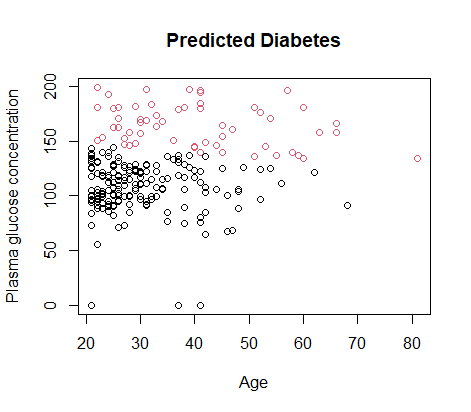
\includegraphics{"C:/Users/Ana/Documents/LiU University/Machine Learning/Lab solutions/ML_lab1/plots for labs/predicted diabetes = age vs glucose concentr.png"}
\caption{Plot of Age VS Plasma Glucose Concentration with predictions}
\end{figure}

Training Misclassification Error: 0.261194

The model seems to give good predictions for higher glucose levels.There
is visible overlap where class overlap in 110-150 region of Glucose
Concentration which can lead to missclassification.This is expected, as
logistic regression applies a linear decision boundary, which cannot
capture more complex relationship in this region. We also see that
classification boundary does not differentiate based on age, because the
predictions for younger and older individuals in similar glucose ranges
look similar, so Age as a factor has limited influence.

Probabilistic equation:
\[P(y = 1 | x1, x2) = 1 / (1 + exp(-(intercept + coef_{x1} * x_1 + coef_{x2} * x_2)))\]

\begin{enumerate}
\def\labelenumi{\arabic{enumi}.}
\setcounter{enumi}{2}
\tightlist
\item
  To derive the decision boundary we use the formula for probabilistic
  eq. and then we equate it to 0.5 and that is the treshold for which we
  devide the probabilities. So when we solve that equation for \(x_2\)
  we get:
  \[x_2 = - \frac{intercept}{coef_{x2}} - \frac{coef_{x1}}{coef_{x2}} * x_1\]
\end{enumerate}

\includegraphics{"C:/Users/Ana/Documents/LiU University/Machine Learning/Lab solutions/ML_lab1/plots for labs predicted values plot with good decision boundary.png"}
Comment whether the decision boundary seems to catch the data
distribution well? The decision boundary cannot perfectly separate the
two classes where they overlap,but it does separate most of the data
appropriately. The slight miscllassification is because of the linear
nature of logistic regression, while actual relationship between
diabetes, Plasma glucose, and Age is probably not perfectly linear so
logistic regression cannot capture it.

\begin{enumerate}
\def\labelenumi{\arabic{enumi}.}
\setcounter{enumi}{3}
\tightlist
\item
  By using these plots, comment on what happens with the prediction when
  r value changes?
\end{enumerate}

\begin{figure}
\centering
\includegraphics{"C:/Users/Ana/Documents/LiU University/Machine Learning/Lab solutions/ML_lab1/plots for labs age vs glucose with r=0.2.png"}
\caption{1. Plot of Age VS Plasma Glucose Concentration using r = 0.2}
\end{figure}

\begin{figure}
\centering
\includegraphics{"C:/Users/Ana/Documents/LiU University/Machine Learning/Lab solutions/ML_lab1/plots for labs age vs glucose with r=0.8.png"}
\caption{1. Plot of Age VS Plasma Glucose Concentration using r = 0.8}
\end{figure}

When the r value changes we classify more or less points as diabetic or
non-diabetic. We notice that the decision boundary that was calculated
will fit more with the higher r value (r=0.8). Higher r value will also
predict more false negatives and fewer false positives. Training
Misclassification Error(r=0.2): 0.369403 Training Misclassification
Error(r=0.8): 0.3078358

\begin{enumerate}
\def\labelenumi{\arabic{enumi}.}
\setcounter{enumi}{4}
\tightlist
\item
  What can you say about the quality of this model compared to the
  previous logistic regression model? How have the basis expansion trick
  affected the shape of the decision boundary and the prediction
  accuracy? Training Misclassification Error, Base Expansion: 0.2406716
  Training Misclassification Error, Original: 0.261194 The decision
  boundary for the basis expanded model seems non-linear, as the
  additional features allow the model to capture more complex
  relationships between \(x_1\)(Plasma glucose) and \(x_2\)(Age). We can
  see that the misclassification error for basis expansion is lower
  compared to the misclassification of the original model, since the
  non-linear boundary better captures the structure of the data. We
  should also mention that there is now a slight risk of overfitting if
  the dataset is noisy
\end{enumerate}

\begin{Shaded}
\begin{Highlighting}[]
\NormalTok{\#\#\#\#\#\#\#\#\#\#\#\#\#\#\#\#\#\#\#\#\#\#\#Q1\#\#\#\#\#\#\#\#\#\#\#\#\#\#\#\#\#\#\#\#\#\#\#}

\NormalTok{mydata \textless{}{-} read.csv("C:/Users/Ana/Documents/LiU University/Machine Learning/csv data for labs/Lab 1 data/pima{-}indians{-}diabetes.csv")}

\NormalTok{\#Creating scatterplot}
\NormalTok{plot(x = mydata[, 8], }
\NormalTok{     y = mydata[, 2],}
\NormalTok{     xlab = "Age",}
\NormalTok{     ylab = "Plasma glucose concentration",}
\NormalTok{     main = "Age vs Plasma glucose concentration",}
\NormalTok{     col = as.factor(mydata[, 9]))}

\NormalTok{\#\#\#\#\#\#\#\#\#\#\#\#\#\#\#\#\#\#\#\#\#\#\#Q2\#\#\#\#\#\#\#\#\#\#\#\#\#\#\#\#\#\#\#\#\#\#\#}

\NormalTok{\#Separating into train/test data}

\NormalTok{X = mydata[, c(2, 8)]  }
\NormalTok{y = mydata[, 9]        }


\NormalTok{n = dim(mydata)[1]    }
\NormalTok{set.seed(12345)        }
\NormalTok{id = sample(1:n, floor(n*0.7))  }

\NormalTok{X\_train = X[id, ] }
\NormalTok{colnames(X\_train) = c("Glucose", "Age")}
\NormalTok{y\_train = y[id]        }
\NormalTok{X\_test = X[{-}id, ]  }
\NormalTok{X\_test = as.data.frame(X\_test)}
\NormalTok{colnames(X\_test) = c("Glucose", "Age")}
\NormalTok{y\_test = y[{-}id]        }

\NormalTok{train\_data = data.frame(Glucose = X\_train[, 1], Age = X\_train[, 2], Diabetes = y\_train)}

\NormalTok{\#Training logistic regression model}
\NormalTok{logit\_model = glm(y\_train \textasciitilde{} Glucose + Age,data = train\_data, family = binomial)}
\NormalTok{\#x\_1 is Plasma glucose}
\NormalTok{\#x\_2 is Age}
\NormalTok{summary(logit\_model)}

\NormalTok{\# Extract coefficients}
\NormalTok{intercept = coef(logit\_model)[1]}
\NormalTok{coef\_x1 = coef(logit\_model)[2]  }
\NormalTok{coef\_x2 = coef(logit\_model)[3]  }

\NormalTok{\# Probabilistic equation}
\NormalTok{cat("P(y = 1 | x1, x2) = 1 / (1 + exp({-}(", intercept, "+", coef\_x1, "* x1 +", coef\_x2, "* x2)))\textbackslash{}n")}

\NormalTok{\# Predict probabilities and classify for training set}
\NormalTok{train\_probs = predict(logit\_model, newdata = data.frame(Glucose = X\_train[, 1], Age = X\_train[, 2]), type = "response")}
\NormalTok{train\_preds = ifelse(train\_probs \textgreater{}= 0.5, 1, 0)}
\NormalTok{train\_error = mean(train\_preds != y\_train)}
\NormalTok{cat("Training Misclassification Error:", train\_error, "\textbackslash{}n")}


\NormalTok{\# Predict probabilities and classify for test set}
\NormalTok{test\_probs = predict(logit\_model, newdata = X\_test, type = "response")}
\NormalTok{test\_preds = ifelse(test\_probs \textgreater{}= 0.5, 1, 0)}

\NormalTok{\#Creating new, predict scatterplot}
\NormalTok{plot(x = X\_test[,2], }
\NormalTok{     y = X\_test[,1],}
\NormalTok{     xlab = "Age",}
\NormalTok{     ylab = "Plasma glucose concentration",}
\NormalTok{     main = "Predicted Diabetes",}
\NormalTok{     col = as.factor(test\_preds))}

\NormalTok{\#\#\#\#\#\#\#\#\#\#\#\#\#\#\#\#\#\#\#\#\#\#\#Q3\#\#\#\#\#\#\#\#\#\#\#\#\#\#\#\#\#\#\#\#\#\#\#}
\NormalTok{decision\_boundary \textless{}{-} function(x\_1) \{}
\NormalTok{  {-}(intercept/coef\_x1) {-} (coef\_x2/coef\_x1) * x\_1\}}

\NormalTok{curve(decision\_boundary(x), add = TRUE, col = "blue", lwd = 2)}

\NormalTok{\#\#\#\#\#\#\#\#\#\#\#\#\#\#\#\#\#\#\#\#\#\#\#Q4\#\#\#\#\#\#\#\#\#\#\#\#\#\#\#\#\#\#\#\#\#\#\#}

\NormalTok{\#  r = 0.2}

\NormalTok{\# Predict probabilities and classify for training set}
\NormalTok{train\_probs = predict(logit\_model, newdata = data.frame(Glucose = X\_train[, 1], Age = X\_train[, 2]), type = "response")}
\NormalTok{train\_preds = ifelse(train\_probs \textgreater{}= 0.2, 1, 0)}
\NormalTok{train\_error = mean(train\_preds != y\_train)}
\NormalTok{cat("Training Misclassification Error:", train\_error, "\textbackslash{}n")}


\NormalTok{\# Predict probabilities and classify for test set}
\NormalTok{test\_probs = predict(logit\_model, newdata = X\_test, type = "response")}
\NormalTok{test\_preds = ifelse(test\_probs \textgreater{}= 0.2, 1, 0)}

\NormalTok{\#Creating new, predict scatterplot}
\NormalTok{plot(x = X\_test[,2], }
\NormalTok{     y = X\_test[,1],}
\NormalTok{     xlab = "Age",}
\NormalTok{     ylab = "Plasma glucose concentration",}
\NormalTok{     main = "Predicted Diabetes",}
\NormalTok{     col = as.factor(test\_preds))}



\NormalTok{\#  r = 0.8}

\NormalTok{\# Predict probabilities and classify for training set}
\NormalTok{train\_probs = predict(logit\_model, newdata = data.frame(Glucose = X\_train[, 1], Age = X\_train[, 2]), type = "response")}
\NormalTok{train\_preds = ifelse(train\_probs \textgreater{}= 0.8, 1, 0)}
\NormalTok{train\_error = mean(train\_preds != y\_train)}
\NormalTok{cat("Training Misclassification Error:", train\_error, "\textbackslash{}n")}


\NormalTok{\# Predict probabilities and classify for test set}
\NormalTok{test\_probs = predict(logit\_model, newdata = X\_test, type = "response")}
\NormalTok{test\_preds = ifelse(test\_probs \textgreater{}= 0.8, 1, 0)}

\NormalTok{\#Creating new, predict scatterplot}
\NormalTok{plot(x = X\_test[,2], }
\NormalTok{     y = X\_test[,1],}
\NormalTok{     xlab = "Age",}
\NormalTok{     ylab = "Plasma glucose concentration",}
\NormalTok{     main = "Predicted Diabetes",}
\NormalTok{     col = as.factor(test\_preds))}

\NormalTok{\#\#\#\#\#\#\#\#\#\#\#\#\#\#\#\#\#\#\#\#\#\#\#Q5\#\#\#\#\#\#\#\#\#\#\#\#\#\#\#\#\#\#\#\#\#\#\#}

\NormalTok{\# Defining functions for new features}
\NormalTok{z\_1 \textless{}{-} function(x\_1)\{}
\NormalTok{  x\_1\^{}4}
\NormalTok{\}}

\NormalTok{z\_2 \textless{}{-} function(x\_1,x\_2)\{}
\NormalTok{  (x\_1\^{}3)*(x\_2)}
\NormalTok{\}}

\NormalTok{z\_3 \textless{}{-} function(x\_1,x\_2)\{}
\NormalTok{  (x\_1\^{}2)*(x\_2\^{}2)}
\NormalTok{\}}

\NormalTok{z\_4 \textless{}{-} function(x\_1,x\_2)\{}
\NormalTok{  (x\_1)*(x\_2\^{}3)}
\NormalTok{\}}

\NormalTok{z\_5 \textless{}{-} function(x\_2)\{}
\NormalTok{  x\_2\^{}4}
\NormalTok{\}}

\NormalTok{\# Computing new features for the train dataset}
\NormalTok{train\_data\_base\_exp \textless{}{-} data.frame(}
\NormalTok{  Glucose = X\_train[, 1],}
\NormalTok{  Age = X\_train[, 2],}
\NormalTok{  z1 = z\_1(X\_train[, 1]),}
\NormalTok{  z2 = z\_2(X\_train[, 1], X\_train[, 2]),}
\NormalTok{  z3 = z\_3(X\_train[, 1], X\_train[, 2]),}
\NormalTok{  z4 = z\_4(X\_train[, 1], X\_train[, 2]),}
\NormalTok{  z5 = z\_5(X\_train[, 2]),}
\NormalTok{  Diabetes = y\_train}
\NormalTok{)}

\NormalTok{\# Model with more features}
\NormalTok{logit\_model\_base\_exp = glm(Diabetes \textasciitilde{} Glucose + Age + z1 + z2 + z3 + z4 + z5, data = train\_data\_base\_exp, family = binomial)}
\NormalTok{summary(logit\_model\_base\_exp)}

\NormalTok{\# Predicting probabilities and classifying for the training set}
\NormalTok{train\_probs\_base\_exp \textless{}{-} predict(logit\_model\_base\_exp, newdata = train\_data\_base\_exp, type = "response")}
\NormalTok{train\_preds\_base\_exp \textless{}{-} ifelse(train\_probs\_base\_exp \textgreater{}= 0.5, 1, 0)}
\NormalTok{train\_error\_base\_exp = mean(train\_preds\_base\_exp != y\_train)}
\NormalTok{cat("Training Misclassification Error, Base Expansion:", train\_error\_base\_exp, "\textbackslash{}n")}

\NormalTok{\# Computing new features for the test dataset}
\NormalTok{test\_data\_base\_exp \textless{}{-} data.frame(}
\NormalTok{  Glucose = X\_test[, 1],}
\NormalTok{  Age = X\_test[, 2],}
\NormalTok{  z1 = z\_1(X\_test[, 1]),}
\NormalTok{  z2 = z\_2(X\_test[, 1], X\_test[, 2]),}
\NormalTok{  z3 = z\_3(X\_test[, 1], X\_test[, 2]),}
\NormalTok{  z4 = z\_4(X\_test[, 1], X\_test[, 2]),}
\NormalTok{  z5 = z\_5(X\_test[, 2])}
\NormalTok{)}

\NormalTok{\# Predicting probabilities and classifying for the test set}
\NormalTok{test\_probs\_base\_exp \textless{}{-} predict(logit\_model\_base\_exp, newdata = test\_data\_base\_exp, type = "response")}
\NormalTok{test\_preds\_base\_exp \textless{}{-} ifelse(test\_probs\_base\_exp \textgreater{}= 0.5, 1, 0)}

\NormalTok{\#Creating new, predict scatterplot}
\NormalTok{plot(x = X\_test[,2], }
\NormalTok{     y = X\_test[,1],}
\NormalTok{     xlab = "Age",}
\NormalTok{     ylab = "Plasma glucose concentration",}
\NormalTok{     main = "Predicted Diabetes (Basis Expansion)",}
\NormalTok{     col = as.factor(test\_preds\_base\_exp))}
\end{Highlighting}
\end{Shaded}


\end{document}
